\documentclass[a4paper,12pt]{article}
\usepackage[margin=18mm]{geometry}
\usepackage{tikz}
\usepackage{amsmath}
\newcommand{\pFourCell}[2]{\makebox[#1em][c]{\ensuremath{#2}}}
\pagestyle{empty}
\begin{document}
\section*{Spaltentreue LaTeX-Ausgabe}
\noindent Gleichung: \texttt{sin(sqrt((x+3)/(2+1)))=5} \hfill Zielvariable: \texttt{x} \hfill Profil: \texttt{standard}

\vspace{8mm}
\begin{center}
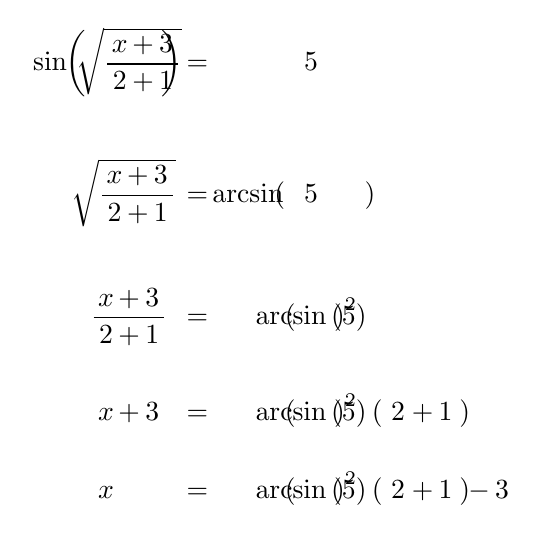
\begin{tikzpicture}[x=1em,y=-1em]
\node[anchor=base, inner sep=0pt] at (3.66,2.9) {$\pFourCell{2.56}{\sqrt{\displaystyle\frac{\pFourCell{0.9}{x}\pFourCell{0.78}{+}\pFourCell{0.88}{3}}{\pFourCell{0.9}{2}\pFourCell{0.78}{+}\pFourCell{0.88}{1}}}}$};
\node[anchor=base, inner sep=0pt] at (0.81,2.9) {$\pFourCell{1.62}{\sin}$};
\node[anchor=base, inner sep=0pt] at (1.81,2.9) {$\pFourCell{0.38}{\left(\vphantom{\pFourCell{2.56}{\sqrt{\displaystyle\frac{\pFourCell{0.9}{x}\pFourCell{0.78}{+}\pFourCell{0.88}{3}}{\pFourCell{0.9}{2}\pFourCell{0.78}{+}\pFourCell{0.88}{1}}}}}\right.}$};
\node[anchor=base, inner sep=0pt] at (5.13,2.9) {$\pFourCell{0.38}{\left.\vphantom{\pFourCell{2.56}{\sqrt{\displaystyle\frac{\pFourCell{0.9}{x}\pFourCell{0.78}{+}\pFourCell{0.88}{3}}{\pFourCell{0.9}{2}\pFourCell{0.78}{+}\pFourCell{0.88}{1}}}}}\right)}$};
\node[anchor=base, inner sep=0pt] at (6.13,2.9) {$=$};
\node[anchor=base, inner sep=0pt] at (10.24,2.9) {$5$};
\node[anchor=base, inner sep=0pt] at (3.47,7.65) {$\pFourCell{2.94}{\sqrt{\displaystyle\frac{\pFourCell{0.9}{x}\pFourCell{0.78}{+}\pFourCell{0.88}{3}}{\pFourCell{0.9}{2}\pFourCell{0.78}{+}\pFourCell{0.88}{1}}}}$};
\node[anchor=base, inner sep=0pt] at (6.13,7.65) {$=$};
\node[anchor=base, inner sep=0pt] at (10.24,7.65) {$\pFourCell{1}{5}$};
\node[anchor=base, inner sep=0pt] at (7.96,7.65) {$\pFourCell{2.04}{\arcsin}$};
\node[anchor=base, inner sep=0pt] at (9.17,7.65) {$\pFourCell{0.38}{\left(\vphantom{\pFourCell{1}{5}}\right.}$};
\node[anchor=base, inner sep=0pt] at (12.31,7.65) {$\pFourCell{0.38}{\left.\vphantom{\pFourCell{1}{5}}\right)}$};
\node[anchor=base, inner sep=0pt] at (3.66,12.075) {$\displaystyle\frac{\pFourCell{0.9}{x}\pFourCell{0.78}{+}\pFourCell{0.88}{3}}{\pFourCell{0.9}{2}\pFourCell{0.78}{+}\pFourCell{0.88}{1}}$};
\node[anchor=base, inner sep=0pt] at (6.13,12.075) {$=$};
\node[anchor=base, inner sep=0pt] at (10.24,12.075) {$\pFourCell{1}{\arcsin\left(5\right)}$};
\node[anchor=base, inner sep=0pt] at (9.55,12.075) {$\pFourCell{0.38}{\left(\vphantom{\pFourCell{1}{\arcsin\left(5\right)}}\right.}$};
\node[anchor=base, inner sep=0pt] at (11.43,12.075) {$\pFourCell{1.38}{\left.\vphantom{\pFourCell{1}{\arcsin\left(5\right)}}\right)^{2}}$};
\node[anchor=base, inner sep=0pt] at (2.83,15.535) {$x$};
\node[anchor=base, inner sep=0pt] at (3.67,15.535) {$+$};
\node[anchor=base, inner sep=0pt] at (4.5,15.535) {$3$};
\node[anchor=base, inner sep=0pt] at (6.13,15.535) {$=$};
\node[anchor=base, inner sep=0pt] at (10.24,15.535) {$\pFourCell{1}{\arcsin\left(5\right)}$};
\node[anchor=base, inner sep=0pt] at (9.55,15.535) {$\pFourCell{0.38}{\left(\vphantom{\pFourCell{1}{\arcsin\left(5\right)}}\right.}$};
\node[anchor=base, inner sep=0pt] at (11.43,15.535) {$\pFourCell{1.38}{\left.\vphantom{\pFourCell{1}{\arcsin\left(5\right)}}\right)^{2}}$};
\node[anchor=base, inner sep=0pt] at (14.21,15.535) {$\pFourCell{1}{2}\pFourCell{0.78}{+}\pFourCell{0.88}{1}$};
\node[anchor=base, inner sep=0pt] at (12.69,15.535) {$\pFourCell{0.38}{\left(\vphantom{\pFourCell{1}{2}\pFourCell{0.78}{+}\pFourCell{0.88}{1}}\right.}$};
\node[anchor=base, inner sep=0pt] at (15.73,15.535) {$\pFourCell{0.38}{\left.\vphantom{\pFourCell{1}{2}\pFourCell{0.78}{+}\pFourCell{0.88}{1}}\right)}$};
\node[anchor=base, inner sep=0pt] at (2.83,18.355) {$x$};
\node[anchor=base, inner sep=0pt] at (6.13,18.355) {$=$};
\node[anchor=base, inner sep=0pt] at (10.24,18.355) {$\pFourCell{1}{\arcsin\left(5\right)}$};
\node[anchor=base, inner sep=0pt] at (9.55,18.355) {$\pFourCell{0.38}{\left(\vphantom{\pFourCell{1}{\arcsin\left(5\right)}}\right.}$};
\node[anchor=base, inner sep=0pt] at (11.43,18.355) {$\pFourCell{1.38}{\left.\vphantom{\pFourCell{1}{\arcsin\left(5\right)}}\right)^{2}}$};
\node[anchor=base, inner sep=0pt] at (14.21,18.355) {$\pFourCell{1}{2}\pFourCell{0.78}{+}\pFourCell{0.88}{1}$};
\node[anchor=base, inner sep=0pt] at (12.69,18.355) {$\pFourCell{0.38}{\left(\vphantom{\pFourCell{1}{2}\pFourCell{0.78}{+}\pFourCell{0.88}{1}}\right.}$};
\node[anchor=base, inner sep=0pt] at (15.73,18.355) {$\pFourCell{0.38}{\left.\vphantom{\pFourCell{1}{2}\pFourCell{0.78}{+}\pFourCell{0.88}{1}}\right)}$};
\node[anchor=base, inner sep=0pt] at (16.31,18.355) {$-$};
\node[anchor=base, inner sep=0pt] at (17.14,18.355) {$3$};
\end{tikzpicture}
\end{center}

\newpage
\section*{Spaltentreue LaTeX-Ausgabe mit Spaltengrenzen}
\vspace{6mm}
\begin{center}
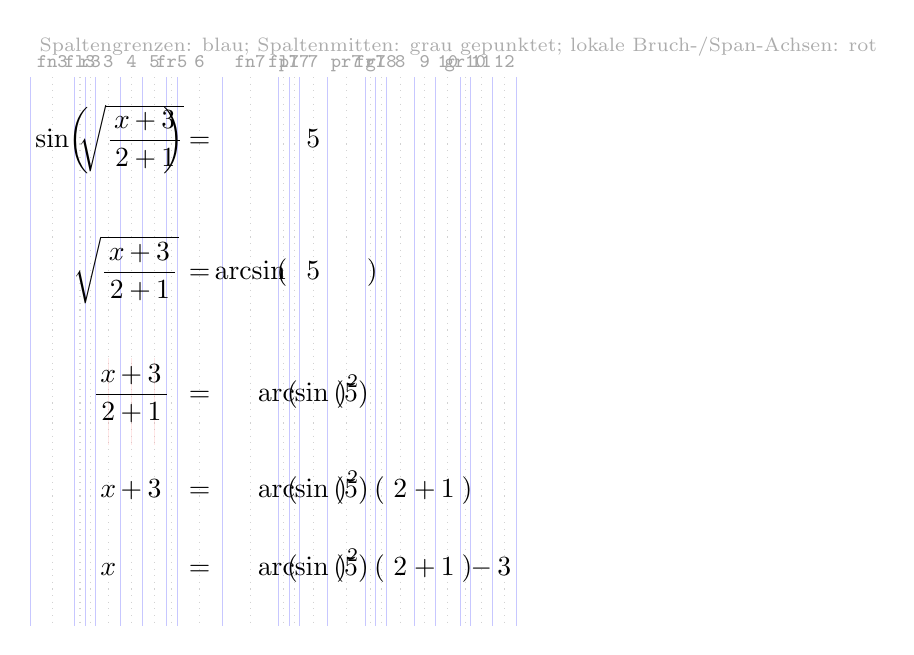
\begin{tikzpicture}[x=1em,y=-1em]
\node[font={\scriptsize}, text=gray!65, anchor=west] at (0,-0.75) {Spaltengrenzen: blau; Spaltenmitten: grau gepunktet; lokale Bruch-/Span-Achsen: rot};
\draw[blue!22, line width=0.28pt] (0,0.35) -- (0,20.19);
\draw[blue!22, line width=0.28pt] (1.62,0.35) -- (1.62,20.19);
\draw[blue!22, line width=0.28pt] (2,0.35) -- (2,20.19);
\draw[blue!22, line width=0.28pt] (2.38,0.35) -- (2.38,20.19);
\draw[blue!22, line width=0.28pt] (3.28,0.35) -- (3.28,20.19);
\draw[blue!22, line width=0.28pt] (4.06,0.35) -- (4.06,20.19);
\draw[blue!22, line width=0.28pt] (4.94,0.35) -- (4.94,20.19);
\draw[blue!22, line width=0.28pt] (5.32,0.35) -- (5.32,20.19);
\draw[blue!22, line width=0.28pt] (6.94,0.35) -- (6.94,20.19);
\draw[blue!22, line width=0.28pt] (8.98,0.35) -- (8.98,20.19);
\draw[blue!22, line width=0.28pt] (9.36,0.35) -- (9.36,20.19);
\draw[blue!22, line width=0.28pt] (9.74,0.35) -- (9.74,20.19);
\draw[blue!22, line width=0.28pt] (10.74,0.35) -- (10.74,20.19);
\draw[blue!22, line width=0.28pt] (12.12,0.35) -- (12.12,20.19);
\draw[blue!22, line width=0.28pt] (12.5,0.35) -- (12.5,20.19);
\draw[blue!22, line width=0.28pt] (12.88,0.35) -- (12.88,20.19);
\draw[blue!22, line width=0.28pt] (13.88,0.35) -- (13.88,20.19);
\draw[blue!22, line width=0.28pt] (14.66,0.35) -- (14.66,20.19);
\draw[blue!22, line width=0.28pt] (15.54,0.35) -- (15.54,20.19);
\draw[blue!22, line width=0.28pt] (15.92,0.35) -- (15.92,20.19);
\draw[blue!22, line width=0.28pt] (16.7,0.35) -- (16.7,20.19);
\draw[blue!22, line width=0.28pt] (17.58,0.35) -- (17.58,20.19);
\draw[gray!35, dotted] (0.81,0.35) -- (0.81,20.19);
\node[font={\ttfamily\scriptsize}, text=gray!70, anchor=base] at (0.81,0) {fn3};
\draw[gray!35, dotted] (1.81,0.35) -- (1.81,20.19);
\node[font={\ttfamily\scriptsize}, text=gray!70, anchor=base] at (1.81,0) {fl3};
\draw[gray!35, dotted] (2.19,0.35) -- (2.19,20.19);
\node[font={\ttfamily\scriptsize}, text=gray!70, anchor=base] at (2.19,0) {r3};
\draw[gray!35, dotted] (2.83,0.35) -- (2.83,20.19);
\node[font={\ttfamily\scriptsize}, text=gray!70, anchor=base] at (2.83,0) {3};
\draw[gray!35, dotted] (3.67,0.35) -- (3.67,20.19);
\node[font={\ttfamily\scriptsize}, text=gray!70, anchor=base] at (3.67,0) {4};
\draw[gray!35, dotted] (4.5,0.35) -- (4.5,20.19);
\node[font={\ttfamily\scriptsize}, text=gray!70, anchor=base] at (4.5,0) {5};
\draw[gray!35, dotted] (5.13,0.35) -- (5.13,20.19);
\node[font={\ttfamily\scriptsize}, text=gray!70, anchor=base] at (5.13,0) {fr5};
\draw[gray!35, dotted] (6.13,0.35) -- (6.13,20.19);
\node[font={\ttfamily\scriptsize}, text=gray!70, anchor=base] at (6.13,0) {6};
\draw[gray!35, dotted] (7.96,0.35) -- (7.96,20.19);
\node[font={\ttfamily\scriptsize}, text=gray!70, anchor=base] at (7.96,0) {fn7};
\draw[gray!35, dotted] (9.17,0.35) -- (9.17,20.19);
\node[font={\ttfamily\scriptsize}, text=gray!70, anchor=base] at (9.17,0) {fl7};
\draw[gray!35, dotted] (9.55,0.35) -- (9.55,20.19);
\node[font={\ttfamily\scriptsize}, text=gray!70, anchor=base] at (9.55,0) {pl7};
\draw[gray!35, dotted] (10.24,0.35) -- (10.24,20.19);
\node[font={\ttfamily\scriptsize}, text=gray!70, anchor=base] at (10.24,0) {7};
\draw[gray!35, dotted] (11.43,0.35) -- (11.43,20.19);
\node[font={\ttfamily\scriptsize}, text=gray!70, anchor=base] at (11.43,0) {pr7};
\draw[gray!35, dotted] (12.31,0.35) -- (12.31,20.19);
\node[font={\ttfamily\scriptsize}, text=gray!70, anchor=base] at (12.31,0) {fr7};
\draw[gray!35, dotted] (12.69,0.35) -- (12.69,20.19);
\node[font={\ttfamily\scriptsize}, text=gray!70, anchor=base] at (12.69,0) {gl8};
\draw[gray!35, dotted] (13.38,0.35) -- (13.38,20.19);
\node[font={\ttfamily\scriptsize}, text=gray!70, anchor=base] at (13.38,0) {8};
\draw[gray!35, dotted] (14.27,0.35) -- (14.27,20.19);
\node[font={\ttfamily\scriptsize}, text=gray!70, anchor=base] at (14.27,0) {9};
\draw[gray!35, dotted] (15.1,0.35) -- (15.1,20.19);
\node[font={\ttfamily\scriptsize}, text=gray!70, anchor=base] at (15.1,0) {10};
\draw[gray!35, dotted] (15.73,0.35) -- (15.73,20.19);
\node[font={\ttfamily\scriptsize}, text=gray!70, anchor=base] at (15.73,0) {gr10};
\draw[gray!35, dotted] (16.31,0.35) -- (16.31,20.19);
\node[font={\ttfamily\scriptsize}, text=gray!70, anchor=base] at (16.31,0) {11};
\draw[gray!35, dotted] (17.14,0.35) -- (17.14,20.19);
\node[font={\ttfamily\scriptsize}, text=gray!70, anchor=base] at (17.14,0) {12};
\node[anchor=base, inner sep=0pt] at (3.66,2.9) {$\pFourCell{2.56}{\sqrt{\displaystyle\frac{\pFourCell{0.9}{x}\pFourCell{0.78}{+}\pFourCell{0.88}{3}}{\pFourCell{0.9}{2}\pFourCell{0.78}{+}\pFourCell{0.88}{1}}}}$};
\node[anchor=base, inner sep=0pt] at (0.81,2.9) {$\pFourCell{1.62}{\sin}$};
\node[anchor=base, inner sep=0pt] at (1.81,2.9) {$\pFourCell{0.38}{\left(\vphantom{\pFourCell{2.56}{\sqrt{\displaystyle\frac{\pFourCell{0.9}{x}\pFourCell{0.78}{+}\pFourCell{0.88}{3}}{\pFourCell{0.9}{2}\pFourCell{0.78}{+}\pFourCell{0.88}{1}}}}}\right.}$};
\node[anchor=base, inner sep=0pt] at (5.13,2.9) {$\pFourCell{0.38}{\left.\vphantom{\pFourCell{2.56}{\sqrt{\displaystyle\frac{\pFourCell{0.9}{x}\pFourCell{0.78}{+}\pFourCell{0.88}{3}}{\pFourCell{0.9}{2}\pFourCell{0.78}{+}\pFourCell{0.88}{1}}}}}\right)}$};
\node[anchor=base, inner sep=0pt] at (6.13,2.9) {$=$};
\node[anchor=base, inner sep=0pt] at (10.24,2.9) {$5$};
\node[anchor=base, inner sep=0pt] at (3.47,7.65) {$\pFourCell{2.94}{\sqrt{\displaystyle\frac{\pFourCell{0.9}{x}\pFourCell{0.78}{+}\pFourCell{0.88}{3}}{\pFourCell{0.9}{2}\pFourCell{0.78}{+}\pFourCell{0.88}{1}}}}$};
\node[anchor=base, inner sep=0pt] at (6.13,7.65) {$=$};
\node[anchor=base, inner sep=0pt] at (10.24,7.65) {$\pFourCell{1}{5}$};
\node[anchor=base, inner sep=0pt] at (7.96,7.65) {$\pFourCell{2.04}{\arcsin}$};
\node[anchor=base, inner sep=0pt] at (9.17,7.65) {$\pFourCell{0.38}{\left(\vphantom{\pFourCell{1}{5}}\right.}$};
\node[anchor=base, inner sep=0pt] at (12.31,7.65) {$\pFourCell{0.38}{\left.\vphantom{\pFourCell{1}{5}}\right)}$};
\draw[red!30, opacity=0.32, line width=0.35pt] (2.83,10.5) -- (2.83,13.65);
\draw[red!30, opacity=0.32, line width=0.35pt] (3.67,10.5) -- (3.67,13.65);
\draw[red!30, opacity=0.32, line width=0.35pt] (4.5,10.5) -- (4.5,13.65);
\node[anchor=base, inner sep=0pt] at (3.66,12.075) {$\displaystyle\frac{\pFourCell{0.9}{x}\pFourCell{0.78}{+}\pFourCell{0.88}{3}}{\pFourCell{0.9}{2}\pFourCell{0.78}{+}\pFourCell{0.88}{1}}$};
\node[anchor=base, inner sep=0pt] at (6.13,12.075) {$=$};
\node[anchor=base, inner sep=0pt] at (10.24,12.075) {$\pFourCell{1}{\arcsin\left(5\right)}$};
\node[anchor=base, inner sep=0pt] at (9.55,12.075) {$\pFourCell{0.38}{\left(\vphantom{\pFourCell{1}{\arcsin\left(5\right)}}\right.}$};
\node[anchor=base, inner sep=0pt] at (11.43,12.075) {$\pFourCell{1.38}{\left.\vphantom{\pFourCell{1}{\arcsin\left(5\right)}}\right)^{2}}$};
\node[anchor=base, inner sep=0pt] at (2.83,15.535) {$x$};
\node[anchor=base, inner sep=0pt] at (3.67,15.535) {$+$};
\node[anchor=base, inner sep=0pt] at (4.5,15.535) {$3$};
\node[anchor=base, inner sep=0pt] at (6.13,15.535) {$=$};
\node[anchor=base, inner sep=0pt] at (10.24,15.535) {$\pFourCell{1}{\arcsin\left(5\right)}$};
\node[anchor=base, inner sep=0pt] at (9.55,15.535) {$\pFourCell{0.38}{\left(\vphantom{\pFourCell{1}{\arcsin\left(5\right)}}\right.}$};
\node[anchor=base, inner sep=0pt] at (11.43,15.535) {$\pFourCell{1.38}{\left.\vphantom{\pFourCell{1}{\arcsin\left(5\right)}}\right)^{2}}$};
\node[anchor=base, inner sep=0pt] at (14.21,15.535) {$\pFourCell{1}{2}\pFourCell{0.78}{+}\pFourCell{0.88}{1}$};
\node[anchor=base, inner sep=0pt] at (12.69,15.535) {$\pFourCell{0.38}{\left(\vphantom{\pFourCell{1}{2}\pFourCell{0.78}{+}\pFourCell{0.88}{1}}\right.}$};
\node[anchor=base, inner sep=0pt] at (15.73,15.535) {$\pFourCell{0.38}{\left.\vphantom{\pFourCell{1}{2}\pFourCell{0.78}{+}\pFourCell{0.88}{1}}\right)}$};
\node[anchor=base, inner sep=0pt] at (2.83,18.355) {$x$};
\node[anchor=base, inner sep=0pt] at (6.13,18.355) {$=$};
\node[anchor=base, inner sep=0pt] at (10.24,18.355) {$\pFourCell{1}{\arcsin\left(5\right)}$};
\node[anchor=base, inner sep=0pt] at (9.55,18.355) {$\pFourCell{0.38}{\left(\vphantom{\pFourCell{1}{\arcsin\left(5\right)}}\right.}$};
\node[anchor=base, inner sep=0pt] at (11.43,18.355) {$\pFourCell{1.38}{\left.\vphantom{\pFourCell{1}{\arcsin\left(5\right)}}\right)^{2}}$};
\node[anchor=base, inner sep=0pt] at (14.21,18.355) {$\pFourCell{1}{2}\pFourCell{0.78}{+}\pFourCell{0.88}{1}$};
\node[anchor=base, inner sep=0pt] at (12.69,18.355) {$\pFourCell{0.38}{\left(\vphantom{\pFourCell{1}{2}\pFourCell{0.78}{+}\pFourCell{0.88}{1}}\right.}$};
\node[anchor=base, inner sep=0pt] at (15.73,18.355) {$\pFourCell{0.38}{\left.\vphantom{\pFourCell{1}{2}\pFourCell{0.78}{+}\pFourCell{0.88}{1}}\right)}$};
\node[anchor=base, inner sep=0pt] at (16.31,18.355) {$-$};
\node[anchor=base, inner sep=0pt] at (17.14,18.355) {$3$};
\end{tikzpicture}
\end{center}
\end{document}
